%!TEX root=qsic2014.tex
% mainfile: qsic2014.tex

% Jeshua Kracht and Jacob Petrovic

\documentclass[conference]{IEEEtran}
%\makeindex
\usepackage{cite}
\usepackage[hidelinks]{hyperref}
\usepackage[cmex10]{amsmath}
\usepackage{eqparbox}
%\usepackage[caption=false]{caption}
%\usepackage[font=footnotesize]{subfig}
\usepackage{url}
\usepackage{mathtools}
\usepackage[pdftex]{graphicx}
\usepackage{caption}
\usepackage{color}

\newcommand{\squishlist}{
 \begin{list}{$\bullet$}
  { \setlength{\itemsep}{0pt}
     \setlength{\parsep}{3pt}
     \setlength{\topsep}{3pt}
     \setlength{\partopsep}{0pt}
     \setlength{\leftmargin}{1.5em}
     \setlength{\labelwidth}{1em}
     \setlength{\labelsep}{0.5em} } }

\newcommand{\squishlisttwo}{
 \begin{list}{$\bullet$}
  { \setlength{\itemsep}{0pt}
     \setlength{\parsep}{0pt}
    \setlength{\topsep}{0pt}
    \setlength{\partopsep}{0pt}
    \setlength{\leftmargin}{2em}
    \setlength{\labelwidth}{1.5em}
    \setlength{\labelsep}{0.5em} } }

\newcommand{\squishend}{
  \end{list}  }

\begin{document}
\title{Empirically Evaluating the Quality of Automatically Generated and Manually Written Test Suites}
% \subtitle{[Extended Abstract]}

\author{\IEEEauthorblockN{Jeshua Kracht, Jacob Z. Petrovic, \\Kristen R. Walcott-Justice}
\IEEEauthorblockA{Department of Computer Science\\
University of Colorado at Colorado Springs\\
Email: \{jkracht, jpetrovi, kjustice\}@uccs.edu}
%\and
%\IEEEauthorblockN{Jacob Z. Petrovic}
%\IEEEauthorblockA{Department of Computer Science\\
%University of Colorado at Colorado Springs\\
%Email: jpetrovi@uccs.edu}
%\and
%\IEEEauthorblockN{Kristen R. Walcott-Justice}
%\IEEEauthorblockA{Department of Computer Science\\
%University of Colorado at Colorado Springs\\
%Email: kjustice@uccs.edu}
\and
\IEEEauthorblockN{Ren\'{e} Just}
\IEEEauthorblockA{Computer Science \& Engineering\\
University of Washington\\
Email: rjust@cs.washington.edu}
\and
\IEEEauthorblockN{Gregory M. Kapfhammer}
\IEEEauthorblockA{Department of Computer Science\\
Allegheny College\\
Email: gkapfham@allegheny.edu}
}

\maketitle
\begin{abstract}

\end{abstract}

%!TEX root=qsic2014.tex
% mainfile: qsic2014.tex

\section{Introduction}
Software testing is a vital task throughout the software development lifecycle for helping to create quality software.  However, the creation and execution of tests is also one of the most expensive components of software development, \textcolor{red}{often comprising of  to \% of the total lifecycle}~\cite{}.  Traditionally, test cases are written manually by the code developers or a quality assurance team.  Unfortunately, manual creation of a high quality test suite requires large amounts of thought, time, and effort. Although manual creation gives developers control over what code is tested and how thoroughly different sections of code is tested,  the cost of the time and effort required to produce these test suites can be extremely high in large projects.  As an alternative to manually writing test cases, many automatic test case generation tools are now available to assist developers in testing code.  However, the quality of the test suites produced by these tools varies, and it is unclear how the test suites of automatic test generation tools compare to those that are manually developed.

%Manual Generated Tests -  benefits vs drawbacks
When manually generating test cases, developers, given time, are able to spend more effort to improve the quality of a test suite to ensure it captures the full depth of the code.  Test focus may vary depending on the developer and project goals/business rules.  Some developers may write tests with the goal of increasing the code coverage, particularly in terms of statements or branches.  Others may focus tests on ``important'' code or code that they expect will be most commonly executed.   In either case, as the program complexity rises, manually writing test cases can become expensive, requiring more thought and labor, when applied to highly complex features~\cite{clarke1998automated}.

An additional challenge in developing test suites is that there is no strict standard or guideline for writing test cases.  Without a standard, test cases are often written inconsistently or subjectively.  While goals or company policy may drive the sections of code that developers attempt to test, the ability of test suites to find bugs is not frequently analyzed.

%Talk about auto generated test suites - benefits vs drawbacks
On the other hand, automatic test case generation tools have been developed to reduce the time and cost of developing a test suite, and some algorithms, in theory, can be used to help improve particular business goals such as coverage or bug finding ability.  Many automatic test suite generators currently exist.  Some are extremely basic, setting up a simple skeleton for methods such as \textcolor{red}{`getters' and `setters' alone}\cite{}.  \textcolor{red}{Others will create slightly more sophisticated skeletons for tests (describe and cite).}  Finally, tools such as CodePro AnalytiX, Palus, TestEra, and Evosuite can generate full, executable test suites that need no modification prior to execution~\cite{Fraser:2011:EAT:2025113.2025179, Zhang:2011:PHA:1985793.1986036, Marinov:2001:TNF:872023.872551, codepro}.  

%Compare Automated vs Manual
Automatic test case generation tools use both deterministic and learning-based algorithms to produce test cases based on particular goals, removing the subjectivity and styles one may find in manually generated tests.  They also significantly reduce the amount of time and effort required of the developer to create the test suite.  However, the quality of the test suites is also of vital concern.  

Test suite quality is frequently measured based on the amount of code covered and on the fault-finding ability of the test suite.  Code coverage is a structure-based criterion that requires the exercising of certain control structures and variables within program~\cite{kapfhammer-testing-handbook}. Fault-based test adequacy criterion, on the other hand, attempts to ensure that the program does not contain the types of faults that are commonly introduced into software systems by programmers~\cite{demillo1978hints, zhu1997software}.  One of the most common types of test quality evaluation in both industry and academic work is based on structurally-based criterion which is commonly analyzed in terms of statement or branch coverage~\cite{weyuker1988evaluation}.

In recent years, mutation testing/scores have been used as another method for evaluating test suite quality. Mutation testing is a fault-based technique which measures the fault-finding effectiveness of test suites on the basis of induced faults~\cite{demillo1978hints, hamlet1977testing}. Mutation testing is a well-known technique to design a new software tests or to evaluate the quality of existing software tests and test suites. The idea of using mutants to measure test suite adequacy was originally proposed by DeMillo et al.~\cite{demillo1978hints}. Mutation testing involves seeding faults in the source program. Each altered version of the source is called a mutant. When a test reveals the mutant then the mutant said to be killed. The ratio of killed mutants/generated mutants is known as the mutation score. In mutation testing, in a simple statement such as  \texttt{if (a < b)}, the \texttt{<} sign will be replaced with all other possible relational operators such as \texttt{>, <=, >= , ==, !=}. The use of mutation operators yields results in the empirical assessment of quality for current testing techniques~\cite{andrews2005mutation}.  

%What we do
In this paper, we analyze existing manually written test suites of open source applications and compare these to test suites that are generated using a two automatic test case generation tools, CodePro and Evosuite, to identify benefits and drawbacks of using automated test suite generation tools.  The three sets of test suites are compared based on the time required to create the test suite, the statement and branch coverage of each test suite, and the mutation score of each test suite.  Although automatic test generation requires far less time and effort than manual test generation, this improvement may not be worthwhile if the quality of the resulting test suites is low in terms of coverage or fault-finding ability.  We additionally examine how the code complexity and lines of code in the original program relate to the code complexity and the lines of code in the tests and the number of test cases generated. Finally, we discuss the overall impact of using automated tools instead of manual test creation.

%Evaluation results
The results indicate stuff.

%contributions
In summary, the main contributions of this paper are as follows:
\squishlist 
\item An examination of the techniques used in sophisticated automatic test case generation tools.
\item An empirical analysis of existing manually written test suites for open source applications.
\item An empirical analysis of automatically generated test suites for open source applications.
\item A comparison of manually written test suites and automatically generated test suites.
\item A discussion of the benefits and drawbacks of using automatic test case generation tools.
\squishend 


%!TEX root=qsic2014.tex
% mainfile: qsic2014.tex

\section{Test Case Generation Techniques}
\label{sec:background}

This section discusses the processes of writing test cases manually and using automatic test case generation tools.  We also describe CodePro and \textsc{EvoSuite}, the automatic test case generation tools that are empirically studied in this paper.

\subsection{Manually Written Tests}

Test suites are most often written manually, either by the developers themselves or through a quality assurance team.  While companies may have their own standards and goals that are followed when writing test cases---such as high levels of statement or branch coverage (e.g.~\cite{DO-178B, IEC61508})---no well-established patterns exist to help standardize test writing practice throughout the software development industry. Thus, the methods and styles of writing individual tests, fulfillment of coverage and fault-finding goals, and the ordering of test suites are often left to industry requirements or personal preference.  

\subsection{Automatically Generated Tests}
Due to the high cost and inconsistencies introduced when developing test suites by hand, automatic test suite generation research is on the rise.  In the past, the writing of test cases was left as an afterthought, and their generation was the responsibility of a separate quality assurance team rather than the developer.  This led to a disconnect between the code and the tests.  In recent years, however, there has been a move towards a more involved test development system in tandem with the the development process ~\cite{Gelperin:1988:GST:62959.62965}.  This movement includes focus on creating unit tests for code as its developed to ensure that code always passing tests thereby improving the quality of the code ~\cite{Canfora:2006:EAT:1159733.1159788}.  Although this improvement in test generation processes successfully increased the reliability of the code, the cost of time and effort to manually write high quality test cases increases as programs became more complex~\cite{clarke1998automated}. 

While many different techniques have been used to automatically generate tests, they can be divided into two key categories: Deterministic and Learning-Based.

\subsubsection{Deterministic}
Deterministic automatic test case generators generally analyze method parameters and basic paths to create unit tests.  The simplest of these tools statically analyze the basic source code paths alone and create skeletons of  needed tests.  For example, JUnitDoclet \cite{JUnitDoclet} uses Javadoc to parse the source code of the application classes. From the collected information, JUnitDoclet writes TestCases and TestSuites where there is a TestSuite for each Java package, a TestCase for each public, non-abstract class, and a skeleton test method for each public method. %The compiler will additionally guide the developer to challenging code segments such as classes that do not have a public constructor, classes that have no default constructors, and accessors for double or float values that need some epsilon when comparing two values.

While these test skeletons are helpful, more sophisticated tools have been developed that create fuller tests by taking the method parameters into consideration. CoView~\cite{CoView}, for example, is a commercial Eclipse plug-in tool that analyzes Java source code and calculates the number of data-driven and cyclomatic paths in a method. Each path is one that should be verified via a unit test. CoView then analyzes existing JUnit tests to determine which paths are being tested and which paths are not tested. This determination is made using instrumented byte code to determine path and branch coverage. CoView then creates missing JUnit test cases for the developer. The developer will have to modify parts of the tests such as the assertions, but the tool can help the developer by identifying the minimum number of unit tests that should be created given parameter options and paths.

Other tools are capable of generating fully executable tests that require no modification.  In this paper, CodePro Analytix is used.  CodePro~\cite{CodePro1} is an Eclipse plug-in tool with many powerful code analysis features and metrics.  Given an input class, the tool creates a corresponding test class complete with multiple test methods for each input class method. The tool analyzes each method and input argument with the goal of generating test cases that exercise each line of code using a combination of both static code analysis and by dynamically executing the code to be tested in order to observe the behavior of the code~\cite{CodePro2}.  CodePro was a Jolt Award finalist and has been analyzed in terms of the types of test cases it can write compared to other tools~\cite{xie2009}.  However, to the best of our knowledge, no work has compared the overall quality of the test cases it creates.

\subsubsection{Learning-Based}
Another set of automatic test case generation tools use learning algorithms to improve the overall quality of the generated test suites.  The two top-ranked tools in this area are Randoop and \textsc{EvoSuite}~\cite{fraser2013a}.  Randoop~\cite{pacheco2007feedback} automatically creates unit tests for Java classes in JUnit format using feedback-directed random test generation. This technique randomly generates sequences of methods and constructor invocations for the classes under test and uses the sequences to create tests. Randoop then executes the sequences it creates and uses the results of the execution to create more assertions, attempting to  avoid redundant and illegal inputs while guiding towards generation of tests that lead to new object states. 

\textsc{EvoSuite}~\cite{fraser:2011:eat:2025113.2025179} , which is used in this paper, ranked first in SBST 2013 Tool Competition~\cite{fraser2013a} and similarly uses a learning algorithm to generate a full, executable test suite.  The tool's evolutionary search approach evolves whole test suites with respect to both coverage and mutation scores.  Optimization with respect to a coverage criterion rather than individual coverage goals helps the algorithm to not be adversely influenced by difficulty of infeasibility of individual coverage goals.  Repeated mutation testing is used to produce a reduced set of assertions that maximizes the number of seeded defects in a class that are revealed by the test cases.


\section{Evaluation}
\label{sec:evaluation}
%----------------------------------------------------------------------------------------------------------------------------------------------------------------------------------------------------------------------------------

\subsection{Key Evaluation Goals}

We are interested in the following research questions.

\textbf{Q1.} Do automated generated unit tests retain the same quality as manually written unit tests?

\textbf{Q2.} What is the cost of time and effort difference in using automated tests versus manually written tests?

\textbf{Q3.} Can developers learn to manually write JUnit tests better with the help of automated generated suites?

\textbf{Q4.} Do Mutation scores and Coverage correlate in any way?

%!TEX root=qsic2014.tex
% mainfile: qsic2014.tex

\subsection{Experiment Design}

%GREG- I stuck to using "we" here because this is the process "we" executed. Is this okay to leave this way?

All experiments were performed on GNU/Linux workstations with kernel 3.2.0-44, a 2 GHzIntel Corporation Xeon E5/Core i7
processor and  15.6 GB of main memory. The unit tests were generated in the Java programming language, for both manual
and automated tests. Figure~\ref{fig:process_diagram}  provides an overview of the test generation implementation with
edges between interacting components. First we identified ten programs
in the SF110~\cite{fraser:2012}. These
programs needed to have manually written test suites for them already to compare to the automated test suites.
Table~\ref{tbl:program_table} provides a list of the selected SF110 programs with their respective lines of code and
cyclomatic complexity.  After identifying these programs, we use the automated test tools \evo and \codepro to
generate test suites. We then took the manual and automated generated test suites and used several different tools to
collect the metrics. MAJOR is used find the mutation score of the program, JaCoCo is used to attain the branch coverage,
and JavaNCSS measures the lines of code and the cyclic complexity of the programs. Time to create the tests was also
recorded manually to compare \evo and \codepro. Time to create the manual tests was available with the SF110.

Because \evo uses a genetic algorithm to generate unit tests, we generated the tests for \evo ten times for each program. With multiple datasets, we can more accurate results with the standard deviation between mutation score, coverage, and time. \codepro uses a deterministic algorithm to generate the tests, so multiple test suite generations were not needed. With results gathered from \evo, \codepro, and the manually written tests, we then compared the scores based upon complexity, time to generate test suite, mutation score, lines of code, and branch coverage.

%GREG\KRISTEN - Here we talk about the graphs and error in statistical analysis. Power symbol ^ is not working for me.
%I'm assuming also we are going to want to include equations for how we calculate R^2 values and the best fit line.
%Do we need a table of results for the R^2 values?

For the graphs, we attempted to find the best fit line to accurately represent to results. It is difficult to find a truly best fit line that gives an overall statistical overlook of the data. This is due to the varying nature of both \evo and the manually written tests. \evo uses a genetic algorithm, which results in varied results for each iteration. This is why as mentioned before, we run ten generations of the test suites and calculate an average for the standard deviation. Manually written test suites are written by different developers. These varying factors result in low  R2 scores, which correlate to how well the best fit line actually represents the data. However, \codepro generated a mutation score of 0 in some cases. We removed these results for \codepro results because it skewed the data in a way that was not graphically indicative of the trends we discovered with \codepro. 

\begin{table}[!t]
\caption{Benchmark Programs and their Properties}
\label{tbl:program_table}
\resizebox{\columnwidth}{!}{%
\begin{tabular}{|l|c|c|}
\hline
\textbf{Program} & \textbf{LOC} &\textbf{Cyclomatic Complexity} \\ \hline
\netweaver                              & 17953                              & 2.82                                                \\ \hline
\inspirento                             & 1769                               & 1.76                                                \\ \hline
\jsecurity                              & 9470                               & 2.05                                                \\ \hline
\saxpath                                & 1441                               & 2.10                                                \\ \hline
\jni                                    & 783                                & 2.05                                                \\ \hline
\xisemele                               & 1399                               & 1.29                                                \\ \hline
\diebierse                              & 1539                               & 1.74                                                \\ \hline
\lagoon                                 & 6060                               & 3.52                                                \\ \hline
\lavalamp                               & 1039                               & 1.50                                                \\ \hline
\jnfe                                   & 1294                               & 1.38                                                \\ \hline
\end{tabular}
}
\end{table}
%JACOB: Put in the text, not the table: "Physical lines of code calculated by JavaNCSS


\begin{figure*}[!t]
\centering
\captionsetup{justification=centering}
  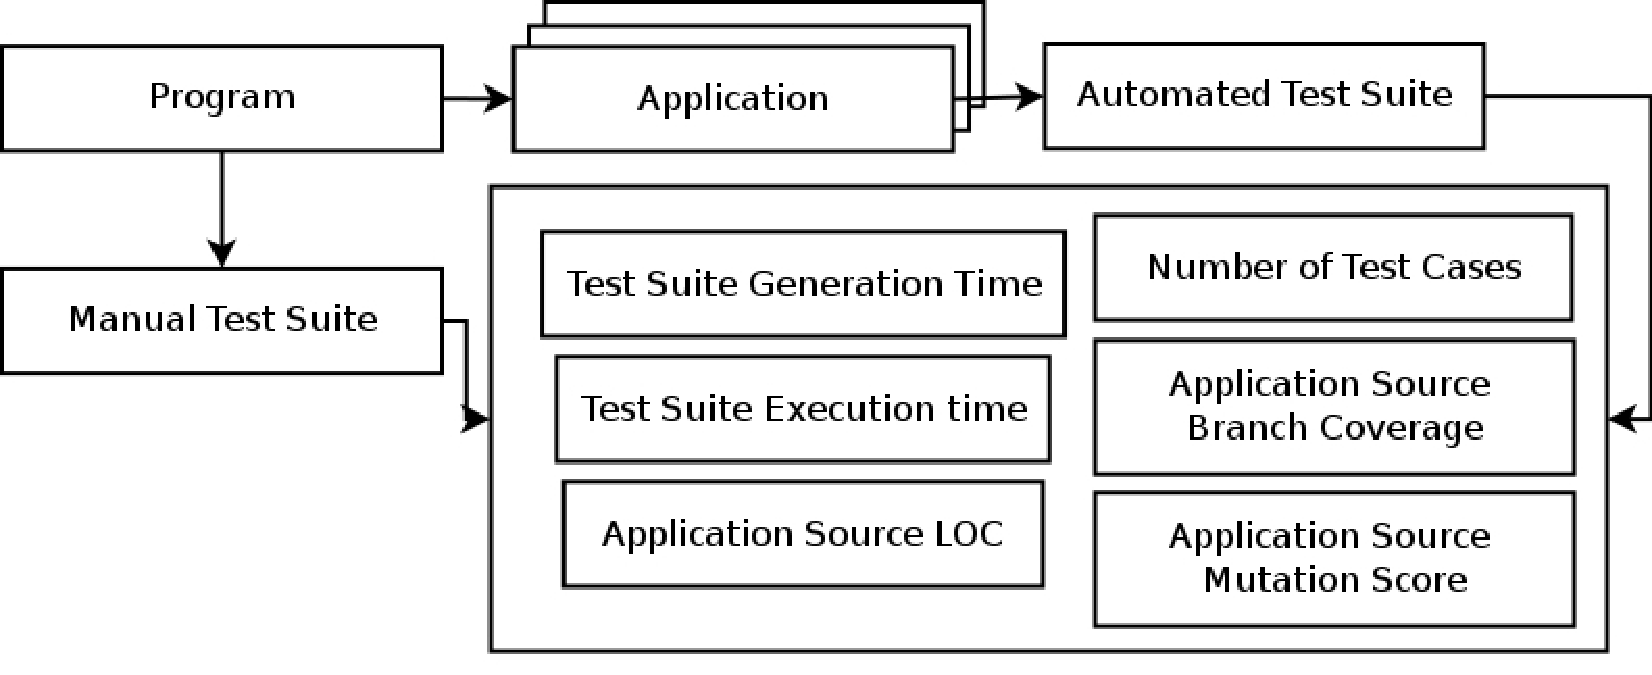
\includegraphics[width=\linewidth]{proccess_diagram.pdf}
    \caption{Test and Mutation Process}
  \label{fig:process_diagram}
\end{figure*}


\subsection{Experiments and Results}
%----------------------------------------------------------------------------------------------------------------------------------------------------------------------------------------------------------------------------------

In the experiments, we first evaluated the time to create each test suite in comparison between Evosuite and CodePro. As shown in Figure ~\ref{fig:Time}, CodePro generated test suites much more quickly than Evosuite did. Although Evosuite consistently takes longer to generate tests regardless of number lines of code and the complexity of the test suite. However, when comparing the complexity of the source code to the time to generate and the complexity of the test suites themselves, there is a clear trade off between time and complexity.

\begin{figure*}[!t]
\centering
  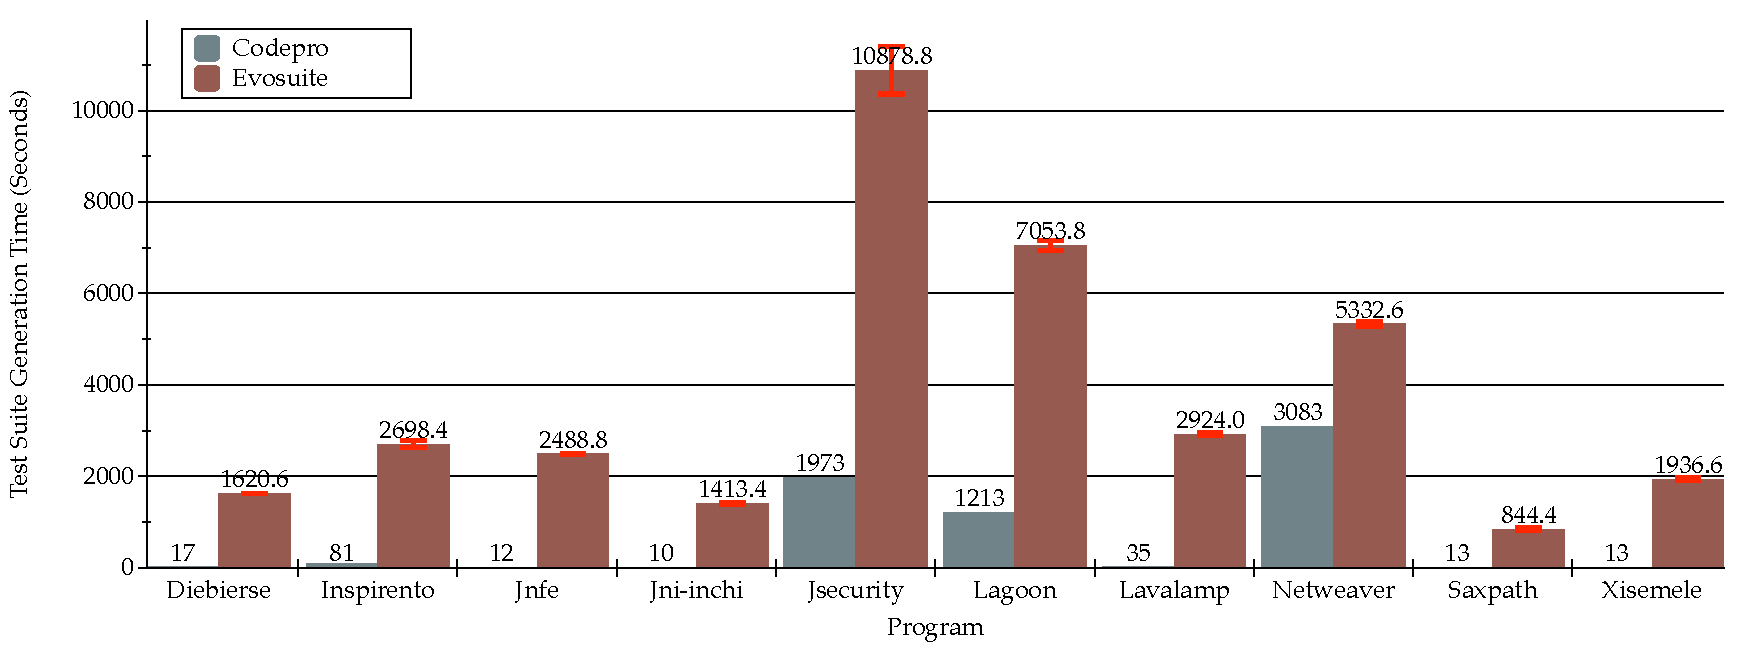
\includegraphics[width=\linewidth]{Time}
    \caption{Time to Generate Test Suite}
  \label{fig:Time}
\end{figure*}

\begin{figure*}[!t]
\centering
  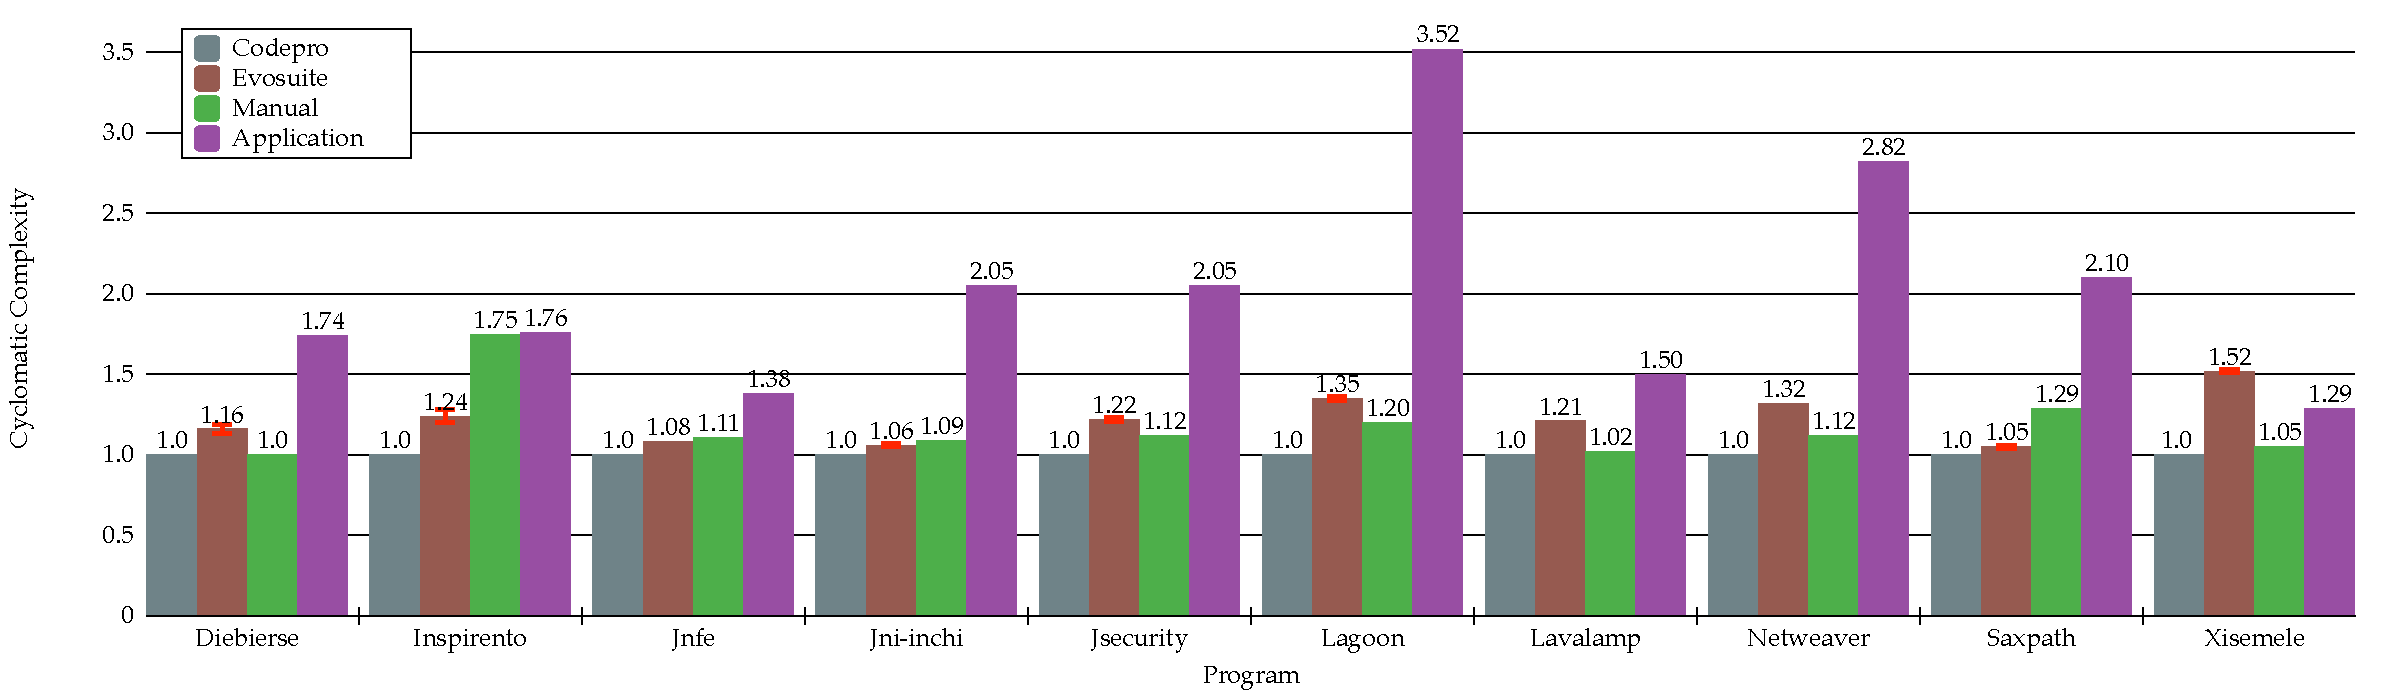
\includegraphics[width=\linewidth]{Complexity}
   \caption{Cyclomatic Complexity of Test Suites and Source Code}
  \label{fig:Complexity}
\end{figure*}

In Figure~\ref{fig:Complexity}, we list the complexities of the source code of the program, and the generated test suites from manual, Evosuite, and CodePro. Note that more complex tests can be more difficult to maintain. The Evosuite test suites are generally more complex than the other two, whereas CodePro is consistently at a lower complexity level. Due to increased complexity of the test suites, it can take more time create and run them~\cite{alspaugh:2007}. As evidenced by Figure~\ref{fig:Time_Complexity}, this indeed seems to be the case. In this data set, it would seem that the more complex the source code is, the more complex the tests are. Furthermore, the more complex the tests are, the longer the test generation takes to complete. This Figure displays the complexity of the test suite versus the time it took to generate the test suite. 

\begin{figure*}[!t]
\centering
  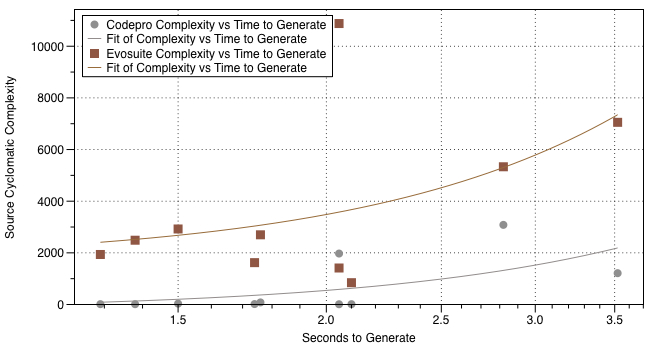
\includegraphics[width=\textwidth]{Time_Complexity}
    \caption{Time to Generate vs. Test Suite Cyclomatic Complexity}
  \label{fig:Time_Complexity}
\end{figure*}


CodePro maintains a low complexity level, but in doing so, this may lead to an inability to address complex code that requires deeper test cases. Although there is a performance boost in the speed to generate the test cases, one must also further examine the quality of the tests that are generated. Evosuite is more complex than the manually generated tests, which may mean that Evosuite cover deeper cases. If the depth of the tests are deeper in Evosuite, than one would expect the mutation scores to increase because the quality of tests would be higher. 

Using mutation scores as a measurement for quality of the tests, we then observe the overall mutation scores given to manual, Evosuite, and CodePro test suites in Figure~\ref{fig:Mutation_Score}. Manual tests generate higher mutation scores in four of the programs, whereas Evosuite also receives higher mutations scores for half of the programs. CodePro receives the highest mutation score for one of the programs by a small margin, but for the rest of the test suites, the scores are the lowest by a large gap. Only in Diebierse did Evosuite vary greatly in the scores received. This indicates that although the average mutation score for Evosuite is within a more unpredictable range of results in one case, on average Evosuite can match the mutation score and quality of the manually written tests.

\begin{figure*}[!t]
\centering
  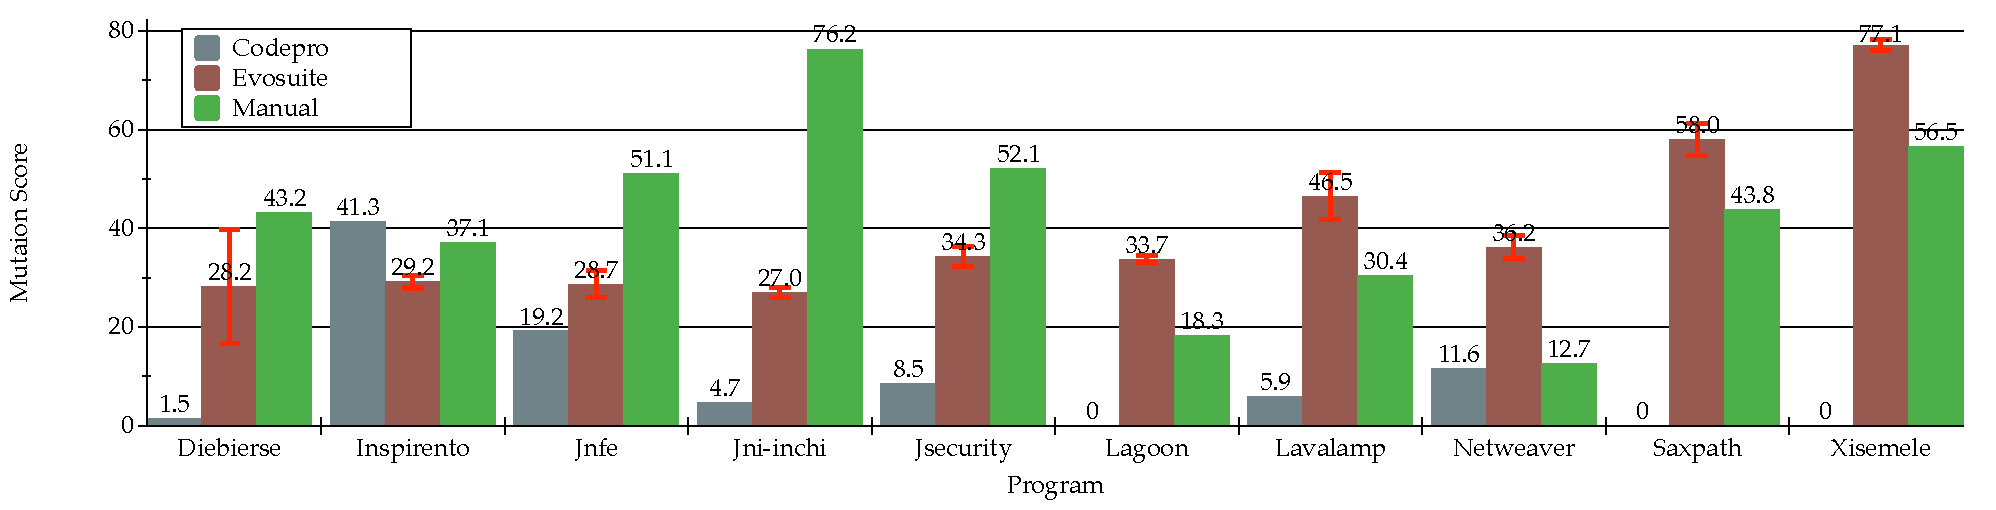
\includegraphics[width=\textwidth]{Mutation_Score}
    \caption{Mutation Score}
  \label{fig:Mutation_Score}
\end{figure*}

To further examine the cause of this, Figure~\ref{fig:Complexity_Mutation}describes the relationships between the mutation score of the test suites and the complexities of the source code. Notice that the manually written tests retain the highest mutation score overall at first. As the complexity of the program increases over time, the the mutation score begins to drop. Around a cyclomatic complexity of 2.3, we find that Evosuite's retains a higher mutation score than manually written tests. CodePro overall receives abysmal mutation scores, and as the cyclomatic complexity of the program increases, the mutation score drops to 0.

This graph is an eye opener to the reality of capturing deeper test cases. Up until a certain point human beings can write deeper test cases to more complex functions. Once the programs become complex, it may be too difficult for a person to cover complex parts of code that require deeper test cases. Evosuite may be at an advantage with its learning algorithm that modifies itself over time to improve the mutation score. With Evosuite seeming to edge out the other two methods in terms of depth, one must also examine the breadth each of the tools can cover as well.

\begin{figure*}[!t]
\centering
  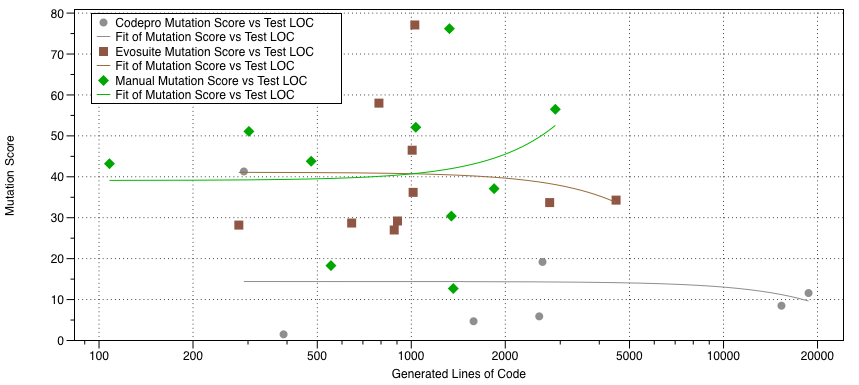
\includegraphics[width=\textwidth]{LOC_Mutation}
    \caption{LOC vs. Mutation Score}
  \label{fig:LOC_Mutation}
\end{figure*}


In Figure~\ref{fig:LOC_Mutation} the relationship between lines of code of the test suite and and mutation score gives an initial impression that automated test suites lack the efficiency of a manually written test suite. CodePro not only results in the lowest mutation scores, but also creates the largest test suites. In the research, we found many of the test cases generated by CodePro were empty and contained comments for developers to put tests into templates. This reveals a different function that CodePro, unlike Evosuite, may be able to provide to developers. 

Although at first glance one may assume that CodePro lacks any usefulness because the quality of tests are low, one could also say that the templates provided by CodePro may give developers the flexibility of modifying and improving the test suite. Evosuite tests are much more complex, and could be conceivably difficult to maintain if the developers wished to evolve the test suite on their own. The trade off between automated and manually written tests could be an argument of modifiability in this case. Although Evosuite scores close to manually written tests when it comes to quality, how would one go about improving the test suites to meet that level depth that manual tests cover in larger programs? The tests would need to be modifiable from a human perspective, which in this case, could be an issue with tests suites like Evosuite.

\begin{figure*}[!t]
\centering
  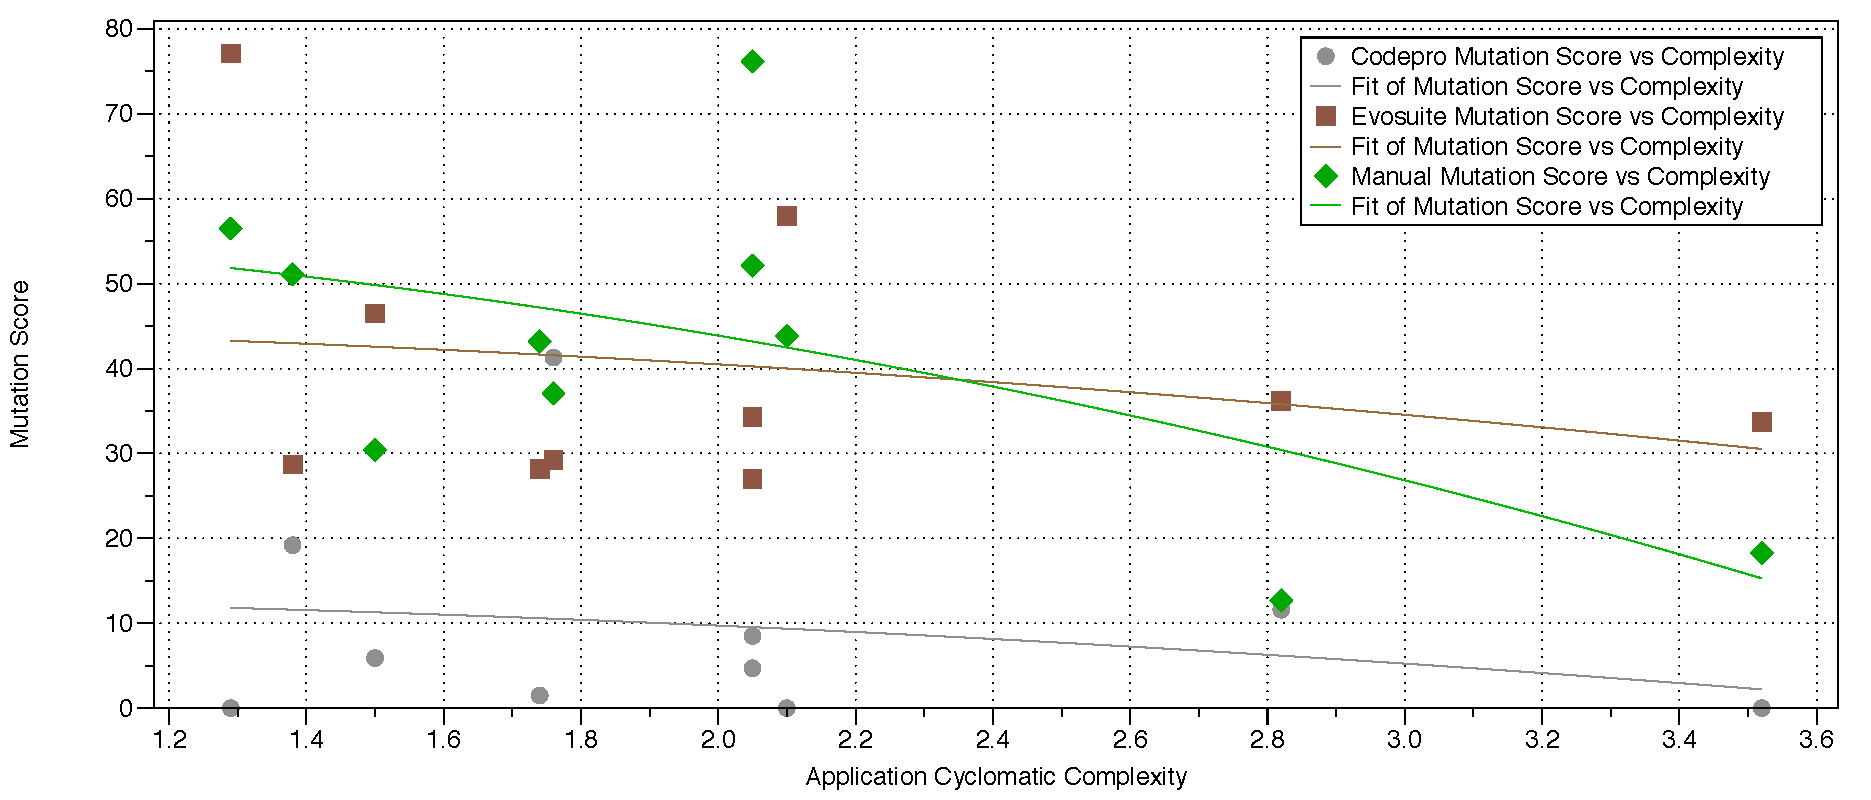
\includegraphics[width=\textwidth]{Complexity_Mutation}
    \caption{Mutation Score vs. Complexity}
  \label{fig:Complexity_Mutation}
\end{figure*}


Depth is important when evaluating the quality of tests, but breadth is an area one must consider when quantifying quality as well, as a test suite that deeply covers just one function will result in little breadth. In Figure~\ref{fig:Coverage},there is an extreme diversity of branch coverage amongst the three evaluated test suites. Overall, CodePro actually scores higher in branch coverage for four of the programs that were tested. Evosuite and the manually generated tests are tied for three programs in scoring the highest branch coverage. For the automated test generators, the branch coverages are closer on average, but manually written test suite scores seem to vary greatly. Again, this is probably due to the inconsistencies in different developers writing their test suites. For example, the developers on Lavalamp could have focused on a TDD philosophy in development, which would predictably yield higher test coverage. However, the developers for Netweaver may have only been concerned with testing one part of their code, and thus branch coverage remained low. In fact, unit tests for only complex parts of the code are common in development, and thus this chart alone only reveals the inconsistent nature of how developers write unit tests. One must look further at the mutation the branch coverage to reach a more definitive 

\begin{figure*}[!t]
\centering
  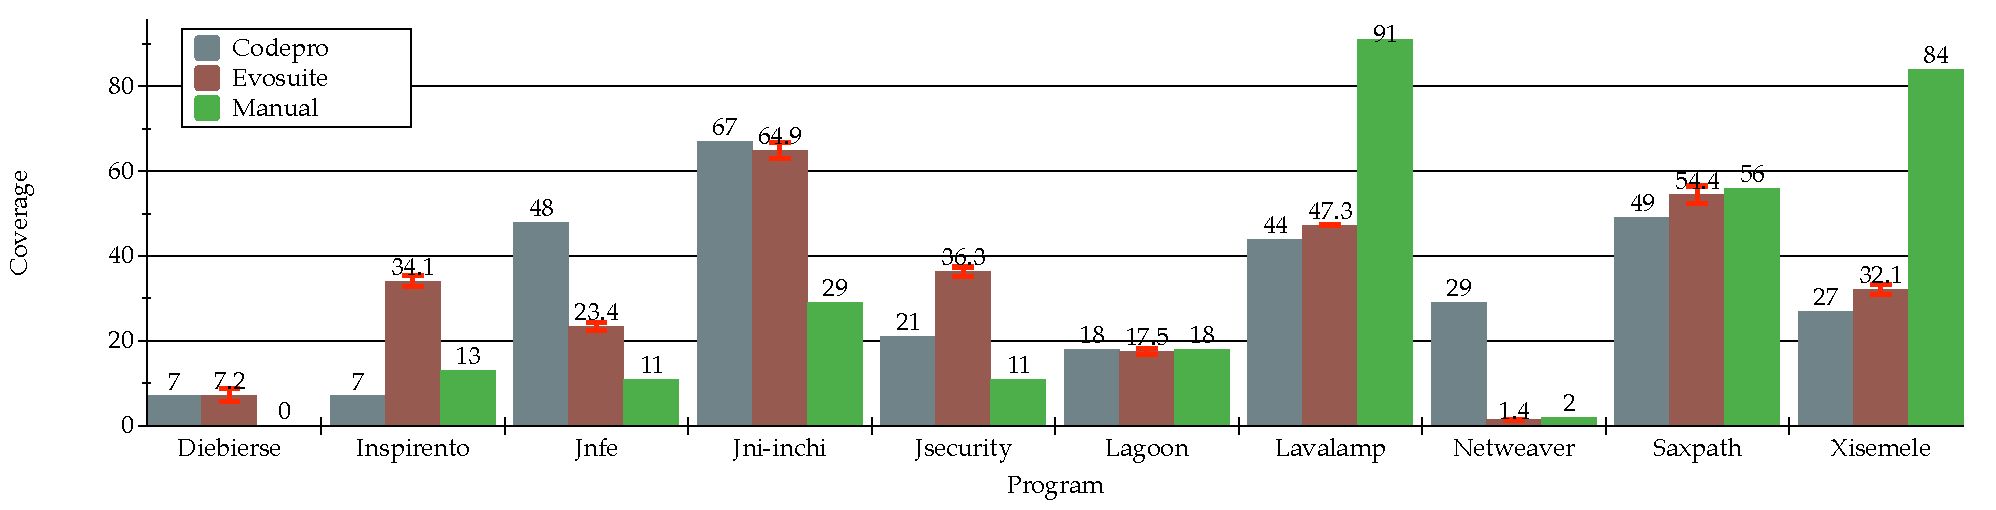
\includegraphics[width=\textwidth]{Coverage}
    \caption{Coverage}
  \label{fig:Coverage}
\end{figure*}

Finally, we examined the center piece of the results, in comparing the evaluation of mutation scores and branch coverage. In Figure~\ref{fig:Coverage_Mutation}, we compare the mutation score (depth) to the branch coverage (breadth) of the test suites. CodePro falls short in the mutation scores, but does have higher branch coverage coverage scores. As the branch coverage increases however, the mutation score in CodePro dips drastically. Understanding that the mutation score was never good to begin with in CodePro, this leads us back to the discussion in perhaps using CodePro as template tool rather than a upfront ready-to-go test suite. Although the mutation scores are low, the coverage is high, providing a large amount of tests for developers to look at and fill over time. 

More interesting are the similar trends between manual and Evosuite generated test suites. Initially Evosuite begins a bit lower in mutation score and branch coverage, but as the branch coverage increases, it would seem that Evosuite surpasses the Manual tests in quality. Overall, the quality of manual tests seems to rise above Evosuite ever so slightly. However, the trends seems to indicate that Evosuite will generate tests that will cover more code with better quality than manually written test suites, although both systems increase in quality as the test branch increases.

\begin{figure*}[!t]
\centering
  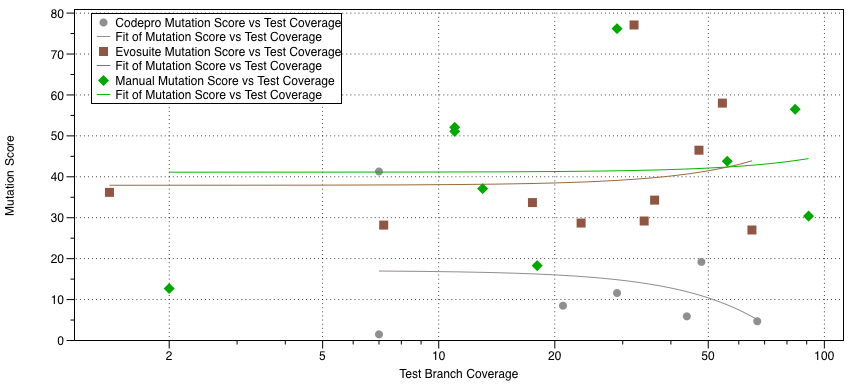
\includegraphics[width=\textwidth]{Coverage_Mutation}
    \caption{Coverage vs. Mutation}
  \label{fig:Coverage_Mutation}
\end{figure*}

\subsection{Threats to Validity}
Measurements in quality of software tests is a subjective measurement. Although mutation score is one way to measure the quality of a test suite, ignoring the human elements of tests are nigh impossible. Developers may need to view tests in order to diagnose faults in the code, and if a developer cannot understand the test they are reading, then the cost of time and effort could be increased on the human part.

The statistical analysis also may be a threat to validity, as the inconsistency in how both Evosuite and manually written tests are created. Also, CodePro generated some test suites with a mutation score of 0, which could mislead one to believing that CodePro has no use for creating quality tests. For this reason we removed these results to give a better impression of the trend CodePro test suites.
%!TEX root=qsic2014.tex
% mainfile: qsic2014.tex

\section{Related Work} \label{sec:related_work}

Since this paper focuses on empirically comparing manually implemented and automatically generated test suites, it is most directly related to Bacchelli et al.'s evaluation of the effectiveness of manual and automated test data generation~\cite{bacchelli2008}. However, there are several distinctions between our paper and this prior work. While the experiments in this paper focus on test suites for ten case study applications, Bacchelli et al.\ only consider select classes that implement data structures like {\tt LRUHashtable}. In contrast to the use of manual tests that were implemented by real-world open-source software developers, the manually-coded test cases in Bacchelli et al.'s were created by the authors themselves.  Moreover, Bacchelli et al.\ use Randoop~\cite{pacheco2007feedback} and JCrasher~\cite{csallner2004}, instead of picking \textsc{EvoSuite}, the current state-of-the-art test data generation tool~\cite{fraser2013a}. Finally, it is important to note that even though Bacchelli et al.\ report coverage and mutation scores, they neither investigate the correlation between coverage and mutation nor perform a comprehensive statistical analysis of the results. In addition, it is possible to make similar comparisons between our paper and the experimental work of Assylbekov et al.~\cite{assylbekov2013}.

The design of the our paper's experiments is informed, in part, by the experimental design and results presented by Inozemtseva and Holmes~\cite{inozemtseva2014}. Like our paper, this prior work also uses real-world programs to empirically investigate the relationship between code coverage and mutation score. However, the primary intent of our work is different than that of Inozemtseva and Holmes: while they investigate the effectiveness correlation for the test suites that come with programs, we consider both manually and automatically generated tests. Moreover, it is important to note that while their paper uses PIT~\cite{pit2014} for fault seeding, our experiments use MAJOR---the only mutation testing tool whose mutants are currently known to be statistically similar to real-world faults~\cite{just2014}.

Our paper's experiments are also partially influenced by the design and results reported on by Gopinath et al.~\cite{gopinath2014}.  This paper is similar to ours because it also investigates the correlation between a test suite's coverage and mutation score.  In addition, Gopinath et al.\ use both manually and automatically generated test suites for more programs than we do; yet, since our experimentation framework is easy to apply to new programs and our presented results demonstrate promise, we will scale our study to Gopinath et al.'s level in future work. Moreover, even though \textsc{EvoSuite} automatically generates better test suites than Randoop~\cite{fraser2013a}---thus motivating its use in our experiments---Gopinath et al.\ use Randoop to create test suites.  In addition, while Gopinath et al.\ employ PIT to seed faults into their case study applications, we decided to use MAJOR since recent results indicate that this tool's faults are a valid substitute for real faults~\cite{just2014}. 

Ultimately, the results from Inozemtseva and Holmes \cite{inozemtseva2014} and Gopinath et al.~\cite{gopinath2014}, in conjunction with those in this paper, present a complementary understanding of the effectiveness of automatically and manually generated test suites. It is also important to remark that, while Just et al.~\cite{just2014} are the first to establish a statistical correlation between a test suite's mutation score and its effectiveness at detecting real-world faults, the purpose of that work is not to develop a full-featured understanding of the quality characteristics of automatically and manually generated test suites---the aim of our paper.

% There are few studies comparing the quality of manual and automated test suites. In one study researchers found that
% using automated test generation tools did not improve the ability to test the software~\cite{fraser2013c}. However, the
% study does not measure the quality of manual and automated generated test suites directly.  Furthermore, only Evosuite
% is used to evaluate the mutations and generate the tests.  This paper expands upon the question of the usefulness of
% automated generated test suites, and if certain systems in generating test suites work better than others.

It is important to note that all of the aforementioned related work focuses of the empirical and technical aspects of test suite effectiveness that are not related to human-centric issues.  In part, our paper was motivated to investigate the complexity and understandability of automatically and manually generated test suites by Fraser et al.'s empirical results revealing that automatically generated tests do not always help software testers find more defects in a program~\cite{fraser2013c}.  While Fraser et al.\ also consider coverage and mutation scores for automatically and manually generated test suites, they only use one automated test suite generator, \textsc{EvoSuite}, while we additionally consider tests created with a deterministic tool called CodePro.

In contrast to our focus on manually and automatically generated test suites for real-world open-source applications, other related work has considered coverage and mutation scores for test suites written by students. For instance, Aaltonen et al.\ observe that automated grading programs may reward students for high-coverage test suites that actually have poor defect-revealing potential~\cite{aaltonen:2010:mav:1869542.1869567}, concluding that a combination of coverage and mutation scores may be the best way to give students accurate feedback on the quality of their test cases.  In addition, Shams and Edwards experimentally observe that mutation scores are lower than coverage values for student-implemented test suites~\cite{shams2013}---a result that corresponds to what we found for open-source programs.

There are a wide variety of past empirical studies that compare different coverage criteria; due to space constraints we
briefly review the most relevant work in this paper. For instance, Frankl et al.\ experimentally compare the all-uses dataflow
criterion to mutation adequacy, finding that, although mutation testing is more expensive that dataflow testing, neither
approach was obviously better than the other~\cite{frankl1997}. As an additional example, Gligoric et al.\ also use
mutation testing to empirically compare the effectiveness of non-adequate test suites that aim to fulfill different
adequacy criteria, revealing that branch coverage and intra-procedural acyclic path coverage are the best
\cite{gligoric2013}.

% Another paper compares measuring quality between faults detection and mutation scores~\cite{just2014}. The research
% statistically proves that mutation score can be used as a test of quality of test suites in place of fault detections.
% The paper uses automated test suites to validate this research, and unlike this paper's research, the author's do not
% compare mutation score, branch coverage, and cyclomatic complexity as joint measurements of quality. 

There is research comparing multiple mutation analysis tools~\cite{ComparingAutomatedMutationTools:2013}. This paper differs from this research in specifically comparing mutation analysis tools for Java. MAJOR was recommended as one one of the premier tools, and was thus used for the evaluation.

\section{Conclusions and Future Work}
\label{sec:conclusion}
%----------------------------------------------------------------------------------------------------------------------------------------------------------------------------------------------------------------------------------
Developers have struggled to find a standard of measuring the quality of tests. Mutation testing and seeding faults has proven as one effective way to identify lower quality tests, and many developers consider high branch coverage a sufficient mark of quality for their test suites. The dilemma becomes a cost trade off between depth and breadth, two measurements that this paper uses to address quality. If mutation analysis results represent the depth of test suites, and branch coverage represents the breadth of test suites, the results of this research identifies trends between the automated tools and developers who write tests. Mutation scores and branch coverage correlate in a positive fashion between the two.

Complexity of the program appeared to also influence the mutation score and time to generate the test suite. In the case of the time needed to generate the test suite, a tool utilizing a genetic algorithm took much longer than a deterministic algorithm to generate test suite. However, the cost of time could be outweighed by the better quality received in the mutation scores. The genetic algorithm sustained a higher mutation score than even the manually written tests when the programs were larger. It may be that automated test tools cover larger programs better than manual tests do.

This paper also addresses new questions. First, what is the purpose of auto generating test suites? CodePro garnered poor scores for both mutation and branch coverage results. Although the quality suffered, the research revealed that the CodePro tests were modifiable. Perhaps some tools could be used assist developers in developing a test suite with a template, placing a focus on modifiable tests rather than a complete test suite to match the quality of manually written tests.

Secondly, what is the future of genetic algorithm based tools such as Evosuite? The tests may not be as modifiable as CodePro's, but the mutation scores in some cases matched and exceeded the mutation scores of manually written tests. If the cost of time and effort given from running Evosuite is less and will generate almost the same results for a large program, perhaps developers ought to consider using a tool like Evosuite.

Finally, the paper identifies the inconsistencies between manually generated tests. There is no way one can say with certainty that the goal of each of the developers for each of the projects was to achieve a high mutation score or high branch coverage. Perhaps developers only care to test one function of the code in depth, or rather they would seek to achieve a high branch coverage. Either way, the intentions of achieving the quality standards outlined in this paper may not be ideal for every developer. 

%GREG\KRISTEN - Will we need something like this?
%In order to reproduce this study and further research in software testing, please reference our material on our web page:

 %http://cs.uccs.edu/~kjustice/QSIC2014/

\bibliographystyle{abbrv}
\bibliography{sample}
%\balancecolumns 

\end{document}
